\documentclass{beamer}


\usetheme{simple}

\usepackage{lmodern}
\usepackage[scale=2]{ccicons}

\usepackage[margin=1cm]{caption}

\usepackage[linesnumbered, ruled]{algorithm2e}
\usepackage{subcaption}
\usepackage{graphicx}
\usepackage[T2A]{fontenc} % enable Cyrillic fonts
\usepackage[english,serbian]{babel}


% TODO: 
%   position adjustement
%   change colours
%       

% Watermark background (simple theme)

\setwatermark{
\includegraphics[height=8cm]{matf_logo1.png}}


\title{Memetski algoritam i njegove primene}
\subtitle{}
\date{\today}
\author{Marica Bogicevic, Boris Karanovic, Petar Kosanin, Filip Sasic}
\institute{Matematicki Fakultet}

\begin{document}

\maketitle


% \begin{frame}[fragile]{Bojenje grafa}
%   \framesubtitle{Memetski algoritam i njegove primene}
  
% \begin{figure}[h!]
% 	\centering

% 	\begin{subfigure}[normla]{0.3\textwidth}
% 		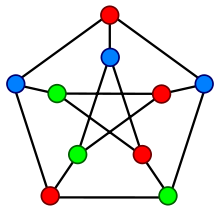
\includegraphics[scale=0.3]{bojene_grafa1}
% 		\caption{Primer ispravnog bojenja cvorova grafa}
% 		\label{bojenje_grafa1}
% 	\end{subfigure}
% 	~
% 	\begin{subfigure}[normla]{0.3\textwidth}
% 		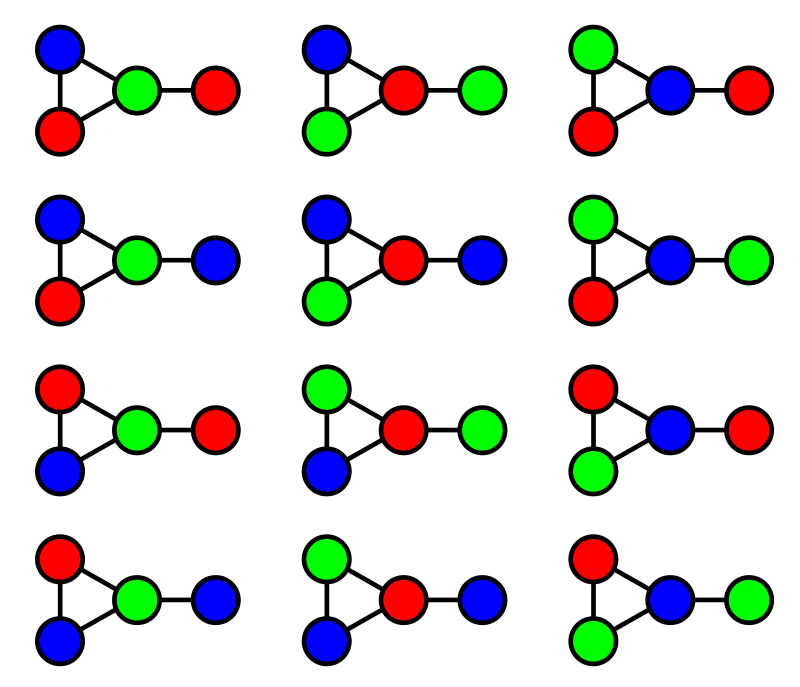
\includegraphics[scale=0.1]{bojenje_grafa2}
% 		\caption{Razlicita ispravna bojenja cvorova grafa}
% 		\label{bojenje_grafa2}
% 	\end{subfigure}
% 		\caption{Slika (a) prikazuje ispravno 3-bojenje Pitersonovog grafa, dok na slici (b) prikazano je 12 razlicitih nacina 3-bojanja grafa. Izvor slika \cite{graph_coloring} }
% \label{bojene_grafa}
% \end{figure}

% \end{frame}

\begin{frame}[fragile]{Problem trgovackog putnika}
  \framesubtitle{Memetski algoritam i njegove primene}
  
   \begin{itemize}
    \item{NP tezak problem, slozenosti O(n!)}
    \item{1932. - Karl Menger definisao pojam ''trgovacki putnik'' }
     \item{Nestandardne karakteristike lokalne pretrage:}
        \begin{itemize}
             \item{Navodena lokalna pretraga}
             \item{Lokalan pretraga sa vise pocetaka}
        \end{itemize}
     \item{Standardna lokalna pretraga se najbolje pokazala}
  \end{itemize}

\end{frame}


\begin{frame}[fragile]{Problem trgovackog putnika}
  \framesubtitle{Memetski algoritam i njegove primene}
  
   \begin{itemize}
    \item{Standardna lokalna pretraga primenjena na roditelje sa verovatnocom Pls}
  \begin{itemize}
    \item{indip = getIterator(Parents);}
     
    \item{If (($Pls \geqslant	 rand(0,1)) \wedge indip \neg best solution$)}
    \item{Apply\_Move(indip);}
     \begin{itemize}
       \item{Modify(indip);}
        \item{If(prevFitness < newFitness)}
        \item{If(random(0,1) > treshold)}
        \item{Accept;}
        \end{itemize}
   \end{itemize}
  \end{itemize}

\end{frame}

\begin{frame}[fragile]{Problem trgovackog putnika}
  \framesubtitle{Memetski algoritam i njegove primene}

    \begin{itemize}
     \item{Modify(indip)}
       \begin{itemize}
     \item{2swap pomeranje}
     \end{itemize}
   
  
    \item{Select\_mating(Parents)}
     \begin{itemize}
     \item{Turnirska selekcija}
     \end{itemize}
       \item{Ukrstanje}
       \begin{itemize}
     \item{Jednopoziciono}
     \end{itemize}
     
     \item{Mutacija}
      \begin{itemize}
     \item{jedinka moze mutirati vise puta u cilju opstanka}
     \end{itemize}
   \item{Select\_Parents(Parents,Offsprings)}
      \begin{itemize}
     \item{$(\mu + \lambda)$ ili $(\mu,\lambda)$ strategija}
     \end{itemize}
  \end{itemize}

\end{frame}


\begin{frame}[fragile]{Bojenje grafa}
  \framesubtitle{Memetski algoritam i njegove primene}

Za neusmeren graf $G = (V, E)$, osnovni memetski algoritam za bojenje grafa ima sledecu formu:
   \begin{itemize}
    \item{Inicijalizacija populacije}
    \item{Kodiranje jedinki}
        \begin{itemize}
            \item Jednu jedinku populacije cini podela skupa $V$ na $k$  disjunktnih podskupova $\{V_1, V_2, ...., V_k\}$
        \end{itemize}
    \item{Lokalna pretraga}
        \begin{itemize}
            \item Tabu pretraga
        \end{itemize}
    \item{Operator ukrstanja}
        \begin{itemize}
            \item GPX(eng. Greedy Partition Crossover)
        \end{itemize}
    \item{Pravilo azuriranja populacije}
  \end{itemize}



\end{frame}




\begin{frame}[fragile]{Bojenje grafa}
  \framesubtitle{Memetski algoritam i njegove primene}

   \begin{itemize}
    \item{Hibridni algoritam za bojenje(HCA)}
    \item{Memetski algoritam za bojenje grafa(MACOL)}
    \item{Hibridni evolutivni algoritam u duetu(HEAD)}
  \end{itemize}
  

\end{frame}


\begin{frame}{Kraj}
  \framesubtitle{Memetski algoritam i njegove primene}

  
\centering
\Huge{Hvala na paznji!}

\end{frame}




\begin{frame}{Kraj}
  \framesubtitle{Memetski algoritam i njegove primene}
\centering
\Huge{Pitanja?}

\end{frame}




\end{document}